% !TeX spellcheck = en_US
\documentclass[aspectratio=169]{beamer}

\usepackage[T1]{fontenc}
\usepackage[utf8]{inputenc}
\usepackage{lmodern}

\usepackage[english]{babel}

\usepackage{amssymb}

\usepackage{minted}
\usepackage{xcolor}
\usepackage{tikz}
\usepackage{amsmath}

\usetikzlibrary{arrows}
\usetikzlibrary{shapes}
\usetikzlibrary{shapes.geometric}

\usetheme{metropolis}


\title[Force-Feedback Teleoperation]{Force-Feedback Teleoperation}
\subtitle{Lab Cognitive Robotics 2020}
\author{Alessandro Riccardi \and Ilyass Taouil \and Benedikt Imbusch}
\institute[RhFWU Bonn]{Rheinische Friedrich-Wilhelms-Universität Bonn}
\date{April 9, 2020}

\newcommand{\fixitemsep}[1]{\setlength{\itemsep}{#1pt}}

\newcommand\FontBig{\fontsize{12}{12}\selectfont}
\newcommand\FontMedium{\fontsize{9}{9}\selectfont}
\newcommand\FontSmall{\fontsize{7}{8}\selectfont}

\begin{document}
\frame[noframenumbering,plain]{
\titlepage
}


\frame{
\frametitle{Table of Contents}
\tableofcontents
}

%TODO rework section names
\section{Introduction and Approach}
\frame{
	\frametitle{Introduction}
	
	\FontBig
	
	\textbf{ANA Avatar XPRIZE}

	\smallskip
	\itshape{"The grand challenge: the ability to physically experience or utilize our skills in another location is restricted by the barriers of time and distance." } \footnote{ANA Avatar XPRIZE (2020). Retrieved from https://avatar.xprize.org/prizes/avatar} %\footnote{avatarxprize}
	
	\bigskip
	\textnormal{
		Force-feedback teleoperation technology
		\begin{itemize}
		\item interaction between two different arms:
			\begin{itemize}
				\item operator arm: Franka Emika Panda
				\item avatar arm: Universal Robots UR10e 
			\end{itemize}
		\end{itemize}
	}
}


\frame{
	\frametitle{Challenges and Approach}
	\begin{itemize}
		\item get the Franka arm end effector pose
		\begin{itemize}
			\item[$\rightarrow$] use the \textit{libfranka} API
		\end{itemize}
		\item control the UR10e
		\begin{itemize}
			\item[$\rightarrow$] use inverse kinematics
			\item[$\rightarrow$] safety measures: joint speed, self collision
		\end{itemize}
		\item robust force sensing on UR10e
		\begin{itemize}
			\item[$\rightarrow$] detection + low-pass filtering of forces from integrated force-torque sensor
		\end{itemize}
		\item force feedback on the Franka arm
		\begin{itemize}
			\item[$\rightarrow$] use the \textit{libfranka} API
		\end{itemize}
		\item apply forces without sensor
		\begin{itemize}
			\item[$\rightarrow$] use a virtual bounding box
		\end{itemize}
	\end{itemize}
}

\frame{
	\frametitle{Challenges and Approach -- Timeline}
	\begin{itemize}
		\item Week 1
		\begin{itemize}
			\item control simulated UR10e in RViz via Franka arm
		\end{itemize}
		\item Week 2
		\begin{itemize}
			\item virtual bounding box for Franka arm
			\item tuning of inverse kinematics, safety measures
			\item implementation force feedback
		\end{itemize}\pause
		\begin{picture}(8,8)
			\put(275,-50){\hbox{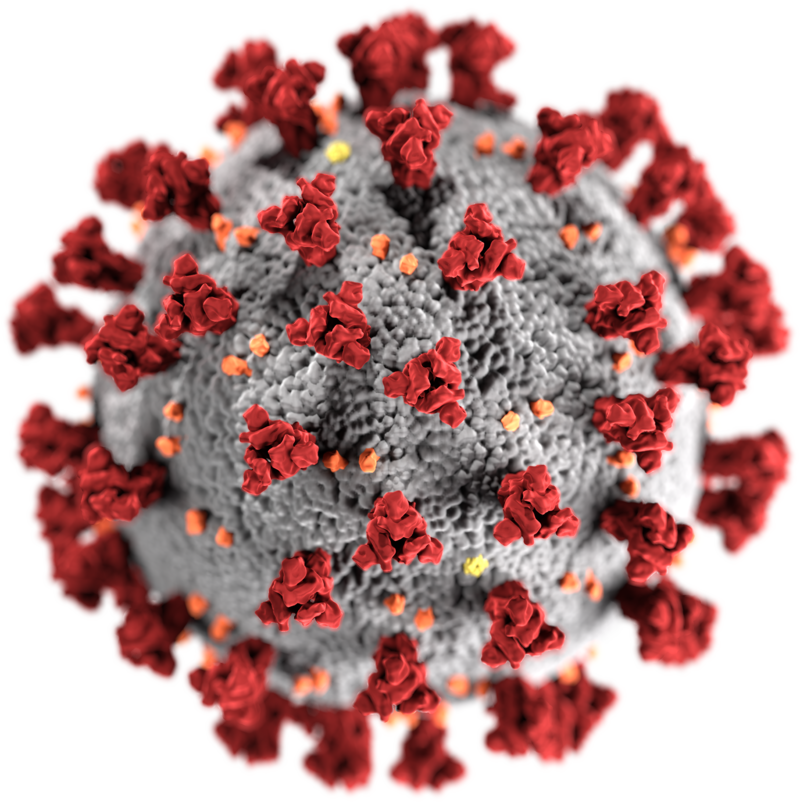
\includegraphics[scale=0.1]{img/corona.png}}}
		\end{picture}
		\item Week 3 (and after)
		\begin{itemize}
			\item \textit{planned: UR10e available for work}
			\item \textit{planned: tuning of force feedback}
			\item \textit{planned: evaluation of performance}
			\item combined simulation of Franka arm and UR10e in RViz
			\item simulated scene with objects $\rightarrow$ collisions, simulated forces
		\end{itemize}
	\end{itemize}
}

\section{Implementation}
\frame{
	\frametitle{Code Architecture}
	\begin{figure}
	    \centering
	    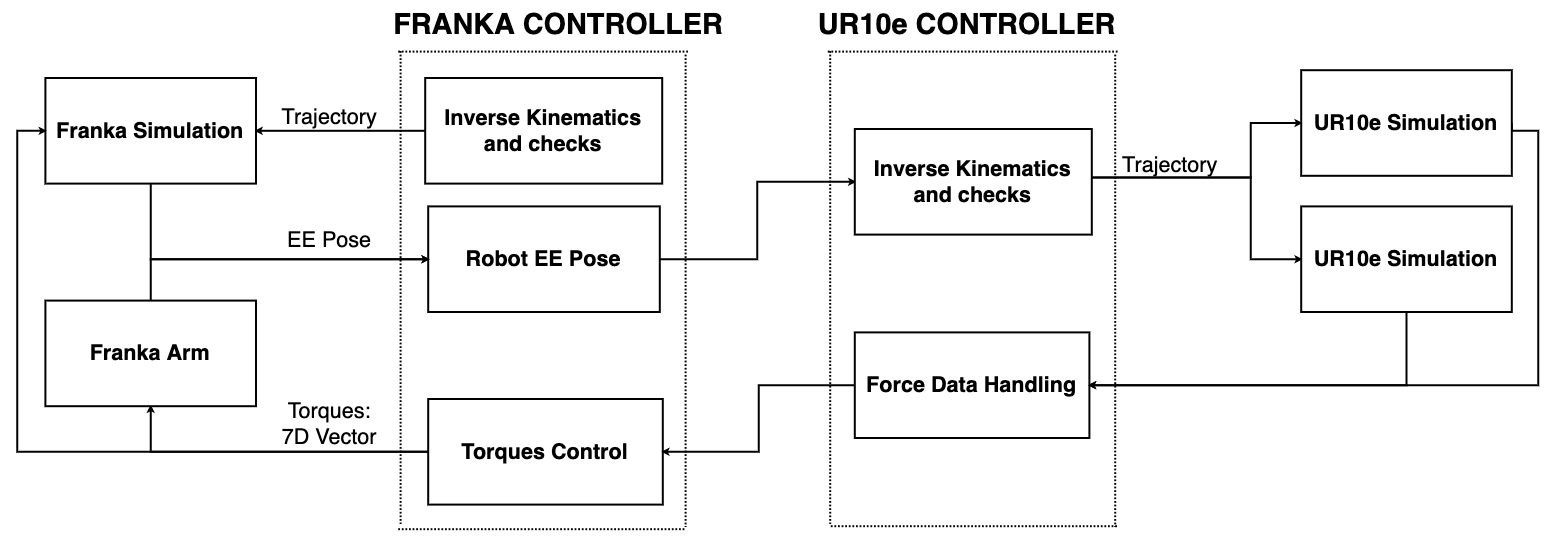
\includegraphics[width=0.9\textwidth]{img/simpler-code-architecture.png}%
	    \vspace{-1em}
	\end{figure}
	
	\FontMedium
    	\begin{columns}
    		\begin{column}{0.5\textwidth}
    			\begin{flushleft}
    				\textbf{Franka Controller Node}
    				\begin{itemize} 
    					\item publish Franka E.E. pose
    					\item perform IK on simulated Franka
    					\item torques control
    				\end{itemize}
    			\end{flushleft}
    		\end{column}
    		\begin{column}{0.5\textwidth}
    			\begin{flushleft}
    				\textbf{UR10e Controller Node}
    				\begin{itemize} 
    					\item perform IK on UR10e
    					\item sanity checks on IK result
    					\item force data handling
    				\end{itemize}
    			\end{flushleft}
    		\end{column}	
	\end{columns}
		
}

\frame{
	\frametitle{Franka API}

	\begin{figure}
		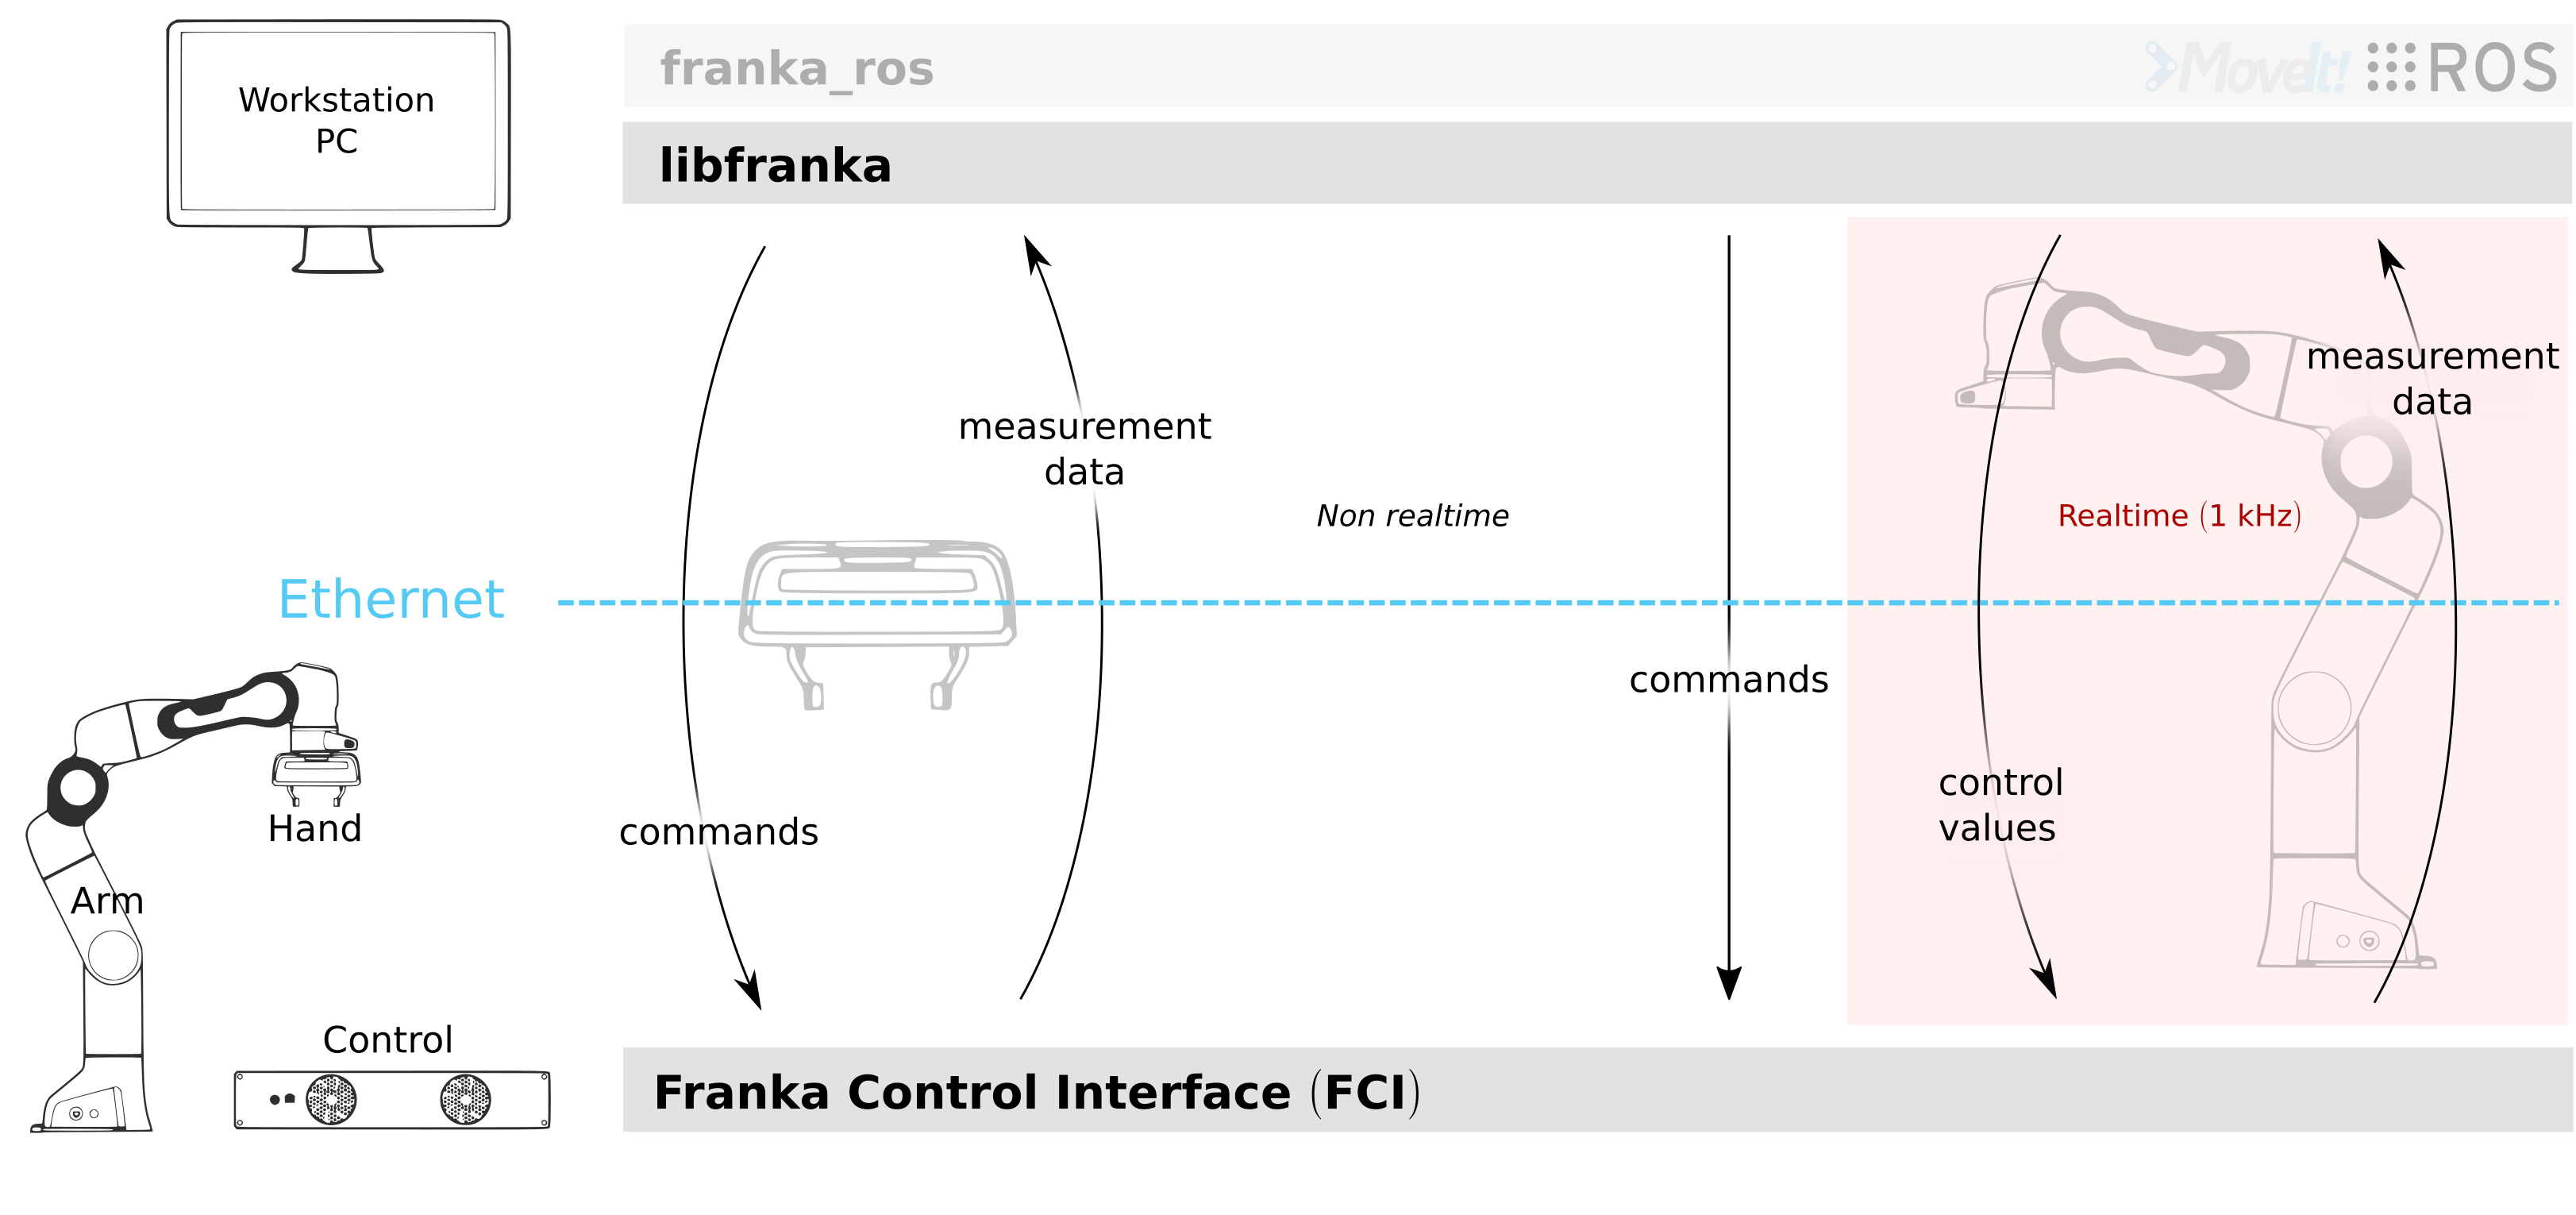
\includegraphics[width=0.7\textwidth]{img/libfranka-architecture.png}%
		\vspace{-1em}
	\end{figure}

	\FontMedium
	\begin{columns}
		\begin{column}{0.4\textwidth}
			\begin{flushleft}
				\textbf{Measurement Data}
				\begin{itemize} 
					\item measured joint data: 
					\begin{itemize} 
						\item position
						\item velocity
					\end{itemize}
				\end{itemize}
			\end{flushleft}
		\end{column}
		\begin{column}{0.4\textwidth}
			\begin{flushleft}
				\textbf{Control Values}
				\begin{itemize} 
					\item controller commands
					\begin{itemize} 
						\item define the torques to be sent to the robot joints
					\end{itemize}
				\end{itemize}
			\end{flushleft}
		\end{column}	
	\end{columns}
 	
}

\frame{
	\frametitle{Inverse Kinematics}
	\begin{itemize}
		\item \textbf{given:} end-effector pose of the Franka arm
		\item \textbf{wanted:} UR10e reaching the same end-effector pose
		\item[$\rightarrow$] \textbf{inverse kinematics:} given robot geometry, \textbf{calculate joint positions}\\such that given end-effector pose is reached
		\vskip24pt
		\item implementation: \textit{NimbRo IK}\footnote{see \textit{Max Schwarz, Anton Milan, Christian Lenz, Aura Muñoz, Arul Selvam Periyasamy, Michael Schreiber, Sebastian Schüller and Sven Behnke: NimbRo Picking: Versatile Part Handling for Warehouse Automation}}
		\item safety measures
		\begin{itemize}
			\item limited joint speed $\rightarrow$ avoid damaging the environment
			\item check for self-collisions before moving the robot
		\end{itemize}
	\end{itemize}
}

\frame{
	\frametitle{Collision Detection}
\vspace{1.2em}
	\begin{columns}[t]
		\begin{column}{0.45\textwidth}
			\textbf{Bounding Box}
			
			\FontMedium
			\begin{itemize}
				\item imaginary finite topological space
				\item specify the limits of Franka arm
			\end{itemize}
			\bigskip
			\textbf{Exceed limit}: computation of closest point to the bounding
			
		\end{column}
	
		
	
		\begin{column}{0.45\textwidth}
			\textbf{Geometry collision}
			
			\FontMedium
			\begin{itemize}
				\item collision detection with geometries
				\item allow an interaction with the world
			\end{itemize}
			\bigskip
			\textbf{Collision}: computation of closest point to the geometry surface
		\end{column}
	\end{columns}

\vspace{1.2em}
\centering
current + closest allowed pose  $\,\to\,$ torques forces

\begin{figure}
	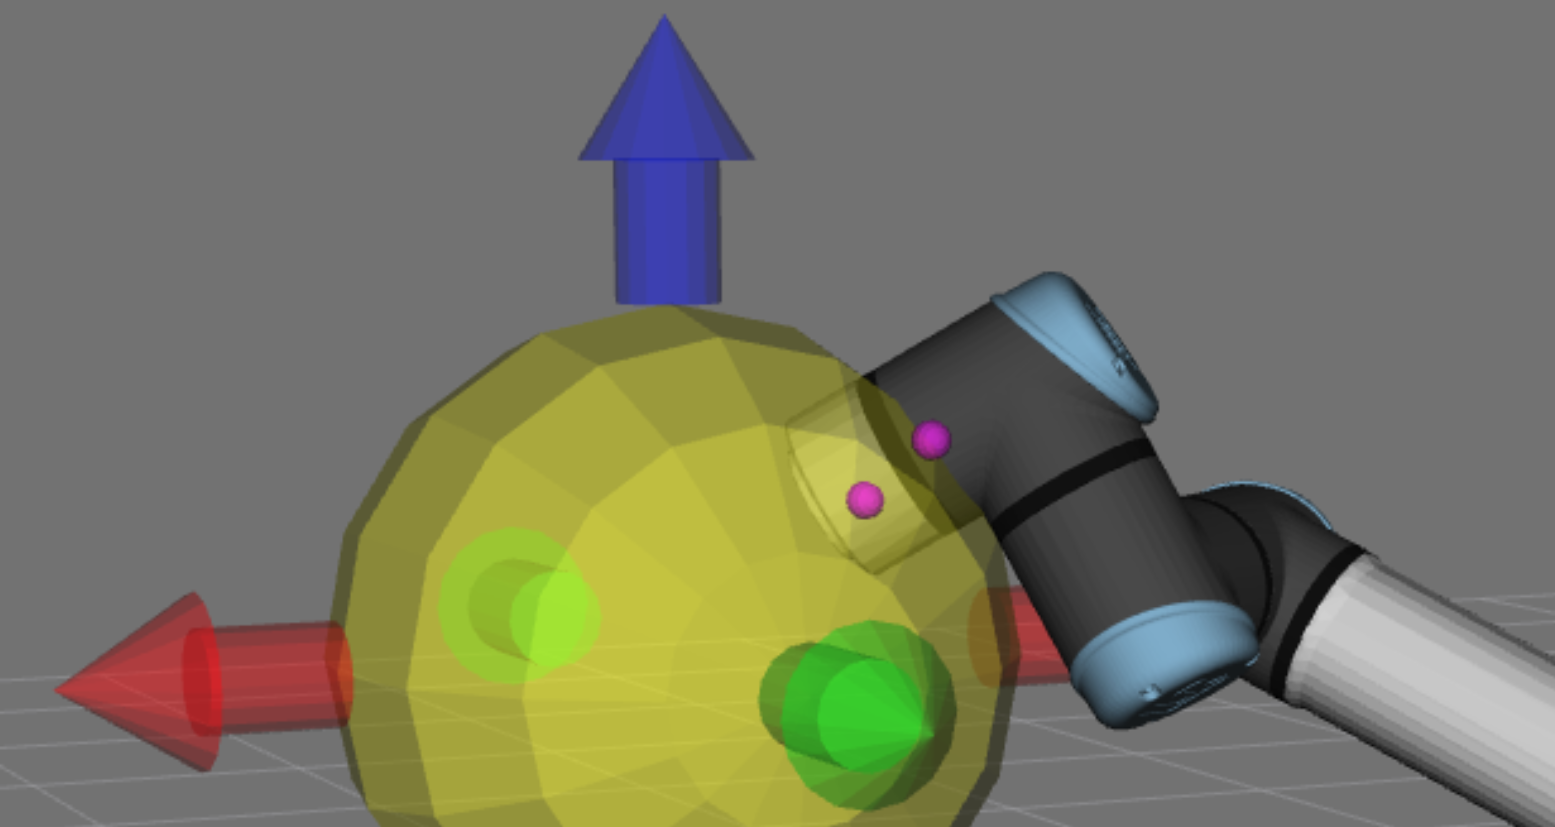
\includegraphics[width=.3\textwidth]{img/ur10e-collision-small.png}%
\end{figure}


}

\frame{
	\frametitle{Force Feedback}
	
	\begin{columns}[t]
		\begin{column}{0.50\textwidth}
			\textbf{Pose Control}
			
			\FontMedium
			\begin{itemize}
				\item used with a bounding box or UR10e simulated
				\item force as a pose difference between collision point and current one
			\end{itemize}
			
			\bigskip
			\bigskip
			\vskip8pt
			
			\textbf{Velocity Compensation}
			\FontMedium
			\begin{itemize}
				\item avoid velocity limits/jumps
				\item joints' acceleration and current velocity
			\end{itemize}	
		\end{column}
	
		\begin{column}{0.50\textwidth}
			\textbf{Wrench Control}
			
			\FontMedium
			\begin{itemize}
				\item used with E.E. forces from UR10e
				\item force directly applied to Franka arm using differentials
			\end{itemize}
			
			\bigskip
			\bigskip
			\vskip6pt

			\textbf{Torques Filtering}
			\FontMedium
			\begin{itemize}
				\item avoid torque limits/jumps
				\item low-pass filter with alpha retention
			\end{itemize}
		
		\end{column}
	\end{columns}
}

\section{Demo}
\frame{
\frametitle{Demo}

\begin{figure}
	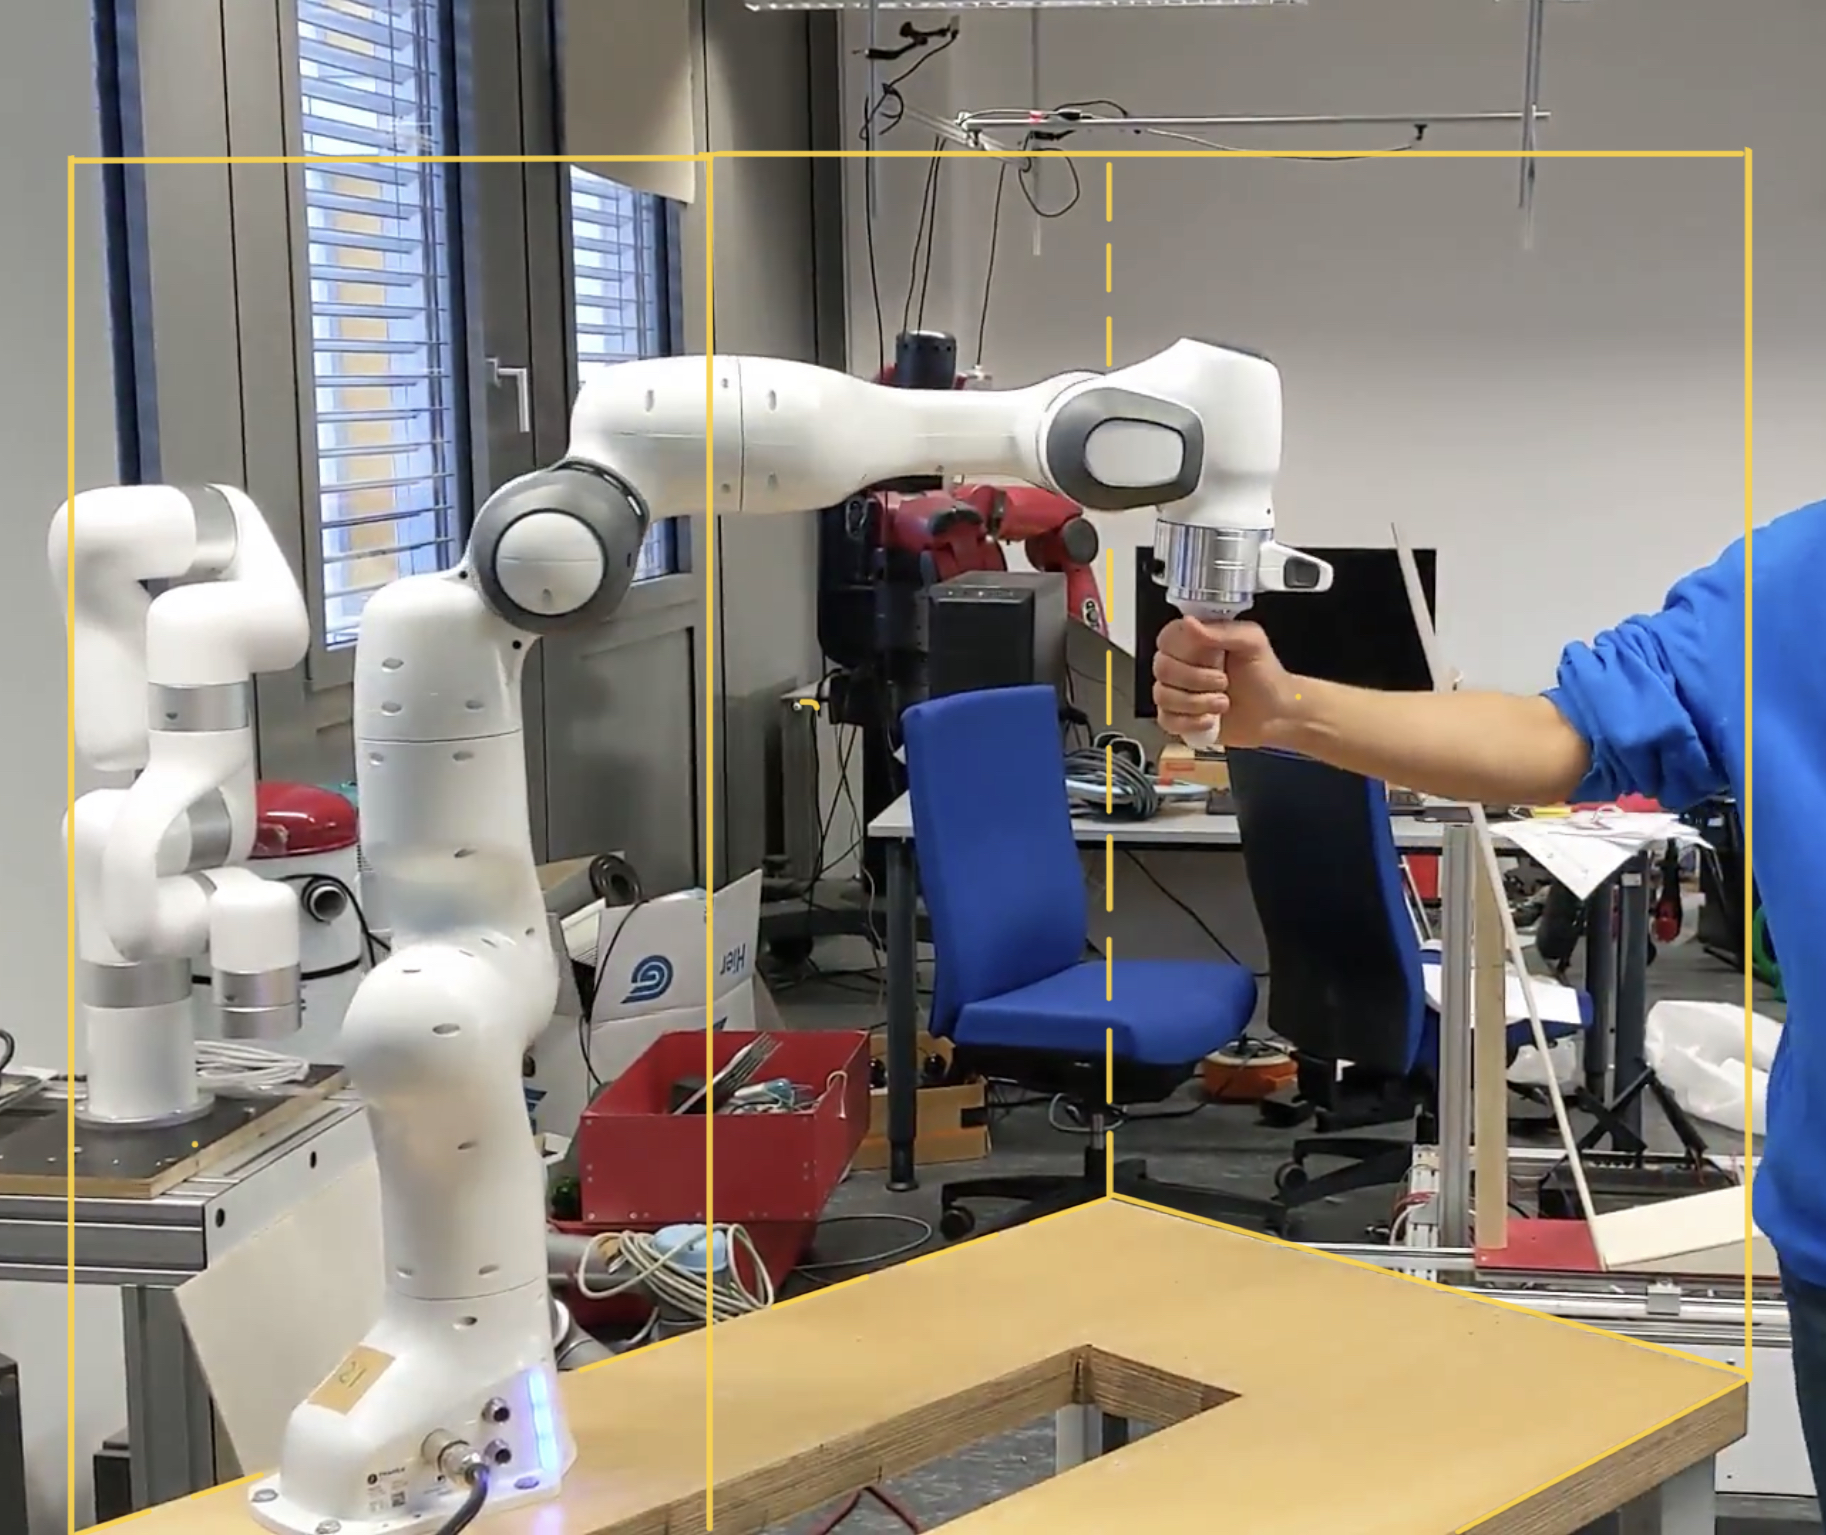
\includegraphics[width=0.5\textwidth]{img/box_pic.jpg}%
\end{figure}
\centering
$\,\to\,$\url{https://tinyurl.com/tfujunc}
}


\frame{
	\frametitle{Conclusion}

	\FontBig

	\textbf{Thank you for your attention!}
}


\end{document}



	
}